\section{Dataset Construction}

In this section, we will introduce the construction of CogBench. 
We will first introduce image collection, annotation and the statistics of CogBench.
Then, we will introduce tasks in CogBench.
% Last, we will show the statistics of CogBench.
% Figure \ref{fig:cogbench} shows an overview of CogBench through an example.


\subsection{Image Collection}

% One of the most important reasons that Cookie Theft picture description task can be widely used as an effective tool to evaluate human cognitive ability is that the picture is carefully designed. \KZ{This sentence is again useless and
% you are repeating yourself.} 
% Therefore, to align with Cookie Theft, images in CogBench are also carefully collected to meet the requirements of picture design in human oriented picture description task as much as possible. \KZ{You can delete this para.}




Based on findings of previous studies \cite{describe-ctp, tasnim-etal-2022-depac}, we set the following image collection criteria: 
% \MY{can you give names to these rules? short and to the point ones, e.g. Rule1 stroy-telling; Rule 2: High information density; ...}

\begin{itemize}
    \item \textbf{Rule 1: Stroy-telling} The image depicts an interesting story clearly. For instance, the Cookie Theft picture tells the story of a mother busy washing dishes while two kids takes the opportunity to stand on a stool and sneakily steal cookies. 
    % Those images simply depict a single event (e.g. a boy is running),  or a scene without a clear story (e.g. a picture of a restaurant) are not considered.
    % \item \textbf{Rule 2}: The image contains one or more subjects (human or animal), engaging in different events.
    % relationships between components
    \item \textbf{Rule 2: Rich Chain-of-Reasonings} Images should display rich Chain-of-Reasonings (CoRs) in a scene. 
    A CoR connects low-level observations in an image to produce a high-level reasoning conclusion or connects the cause and effect of events. 
    For example, ``The mother is busy washing dishes. + The boy is standing on the stool behind the mother. + The girl standing by the boy is shushing him. + The boy is fetching cookies from the jar in the carbinet. $\rightarrow$ The boy and girl are stealing cookies.'' is a CoR about high-level event ``stealing cookies''. Note that the story is actually constructed via these CoRs.
    \item \textbf{Rule 3: Content Complexity Restriction} Images should contain rich content but not be overly complex. The number of subjects should be limited for better emphasis on the key points of the story, facilitating description by humans or models. 
    % For those pictures with a lot of subjects, even they are rich in content and there might be interesting stories in them, it is difficult for models or even humans to describe them in a short time. Therefore, we do not consider these pictures.
\end{itemize}

\begin{figure}[th]
  \centering
  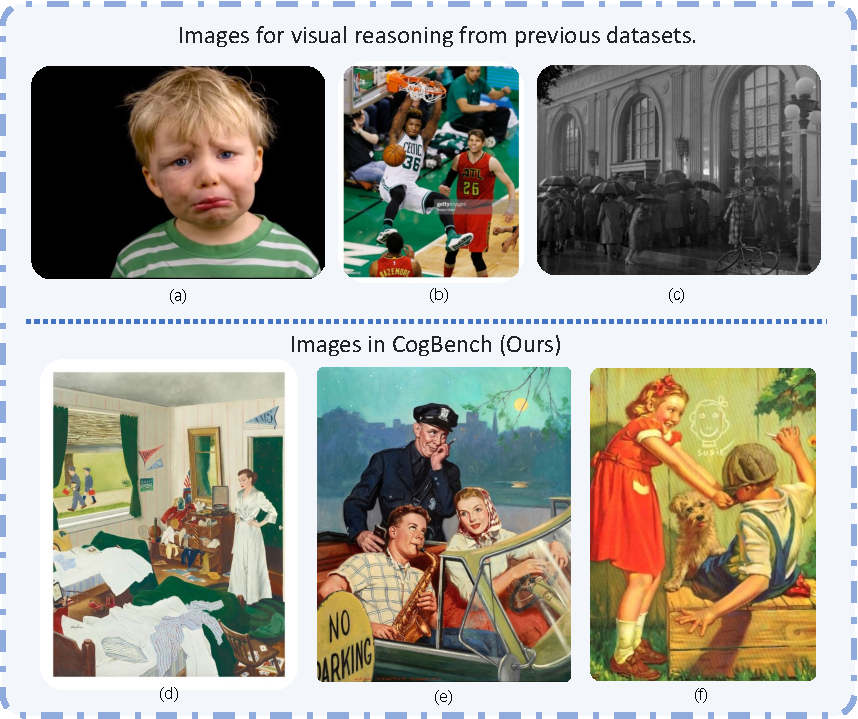
\includegraphics[width=0.45\textwidth]{figs/cog_img_example.pdf}
  \caption{The comparison between our images and those from the previous visual reasoning tasks.
  Compared to our images, image (a) has fewer entities and CoRs, image (b) and (c) have some entities, but fewer CoRs.
  % \MY{can you add elements contrast here? e.g. previous datsets have entity, but few CoRs. The selected pics are not that contrastive (we are trying to say that exsiting datasets involve simple pictures), picture A and C are quite similar to something can be involved in our dataset, where you can infer a lot of things.}
}
  \label{fig:cogbench_example}
\end{figure}



With the above criteria, we aim to select high-quality images for cognition evaluation of LVLMs. 
% Currently, we have collected 95 images for CogBench. 
Most of the images are manully collected from Pinterest\footnote{https://www.pinterest.com/}, and the Cookie Theft is also included in CogBench.
\figref{fig:cogbench_example} illustrates the differences between our images and those from other datasets.
% \MY{We should say how many pics were included first, then screened out by which rule, and ended up with xxx. Do we have an annotation-based filtering as well? Like after annotation, some pics are too simple or too difficult then it's excluded at last.}
% \XJ{As the collection cretiria are strict, we do not filter out too many images.}

\subsection{Image Annotation}
\label{sec:annotation}


\begin{figure*}[h]
  \centering
  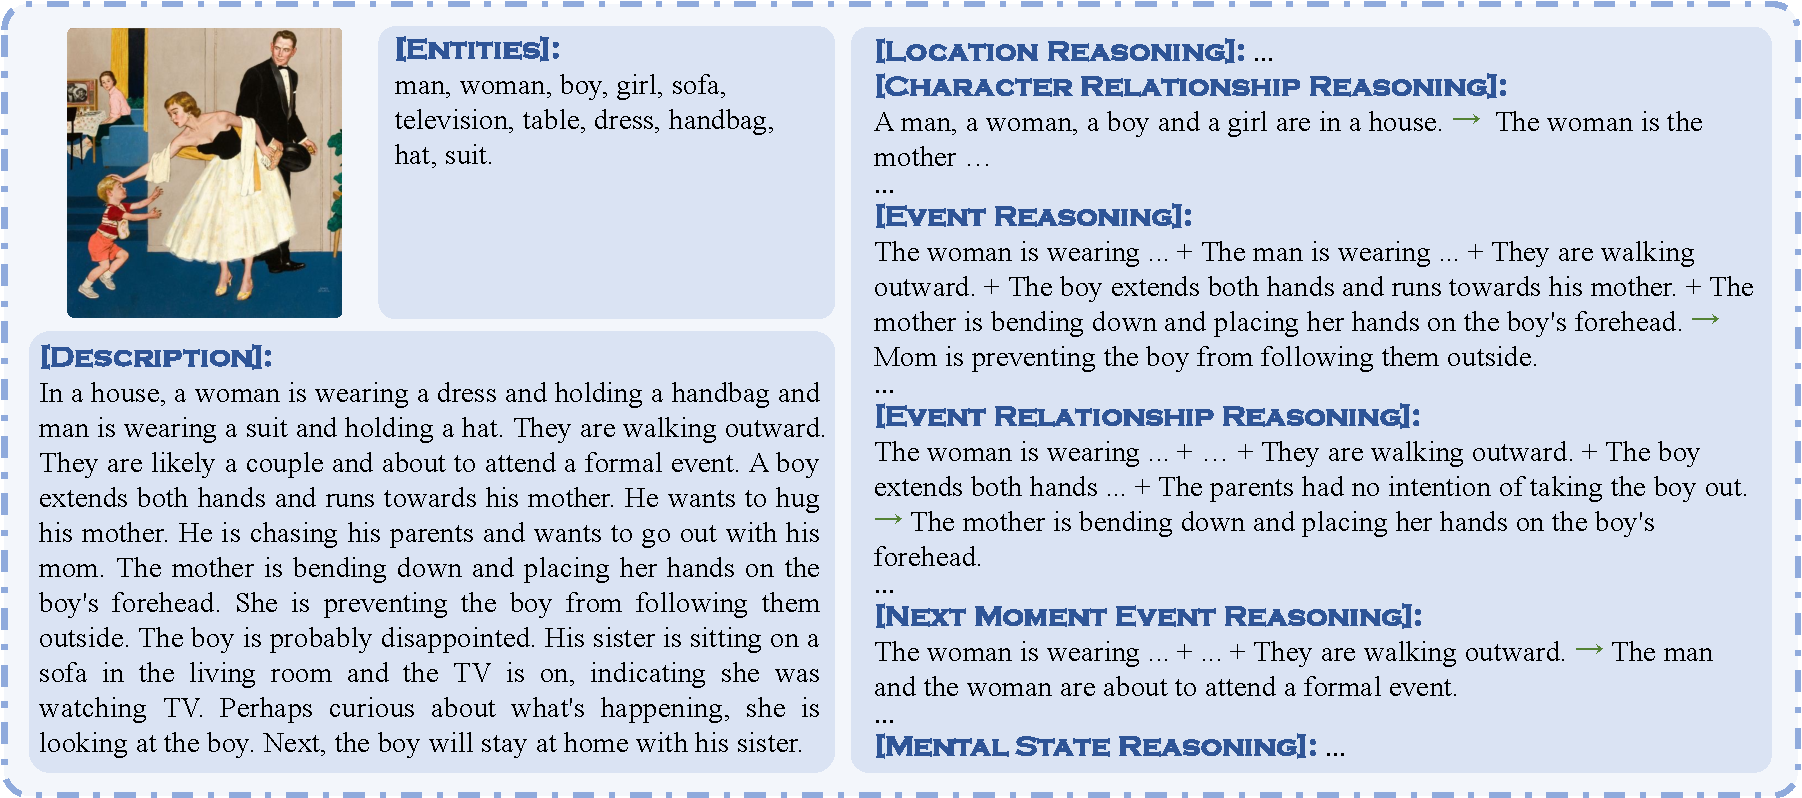
\includegraphics[width=0.95\textwidth]{figs/descrption_task_3.pdf}
  \caption{An example of Description task from CogBench. 
  % \KZ{The fonts are too small.
  % No need to include everything. You can include a complete example in the 
  % appendix.} \MY{separate VQA into another figure, it will simplify this one and make it easier to understand}
  % \XJ{font size increased.}
}
  \label{fig:cogbench}
\end{figure*}


Human annotators, mostly undergraduate or graduate students aged 18-28, are hired to annotate the collected images. 
% The annotators are mostly undergraduate or graduate students with normal cognitive functioning, aged between 18 and 28.
As shown in Figure \ref{fig:cogbench}, the annotation includes three parts: [Entities], [CoRs] and [Description].

By annotating [Entities] and [CoRs], we aim to evaluate the low-level recognition ability and high-level cognitive reasoning ability of models respectively based on description. 
% By annotate , we aim to evaluate the high-level cognitive reasoning ability of models during description. 
% [CoRs] can also be used for generating questions for CogVQA task.
[Description] is annotated as the reference description for the image.
The three parts are annotated in a sequential order.

% [Entities]
\paragraph{Entity Annotation} We ask annotators to list as many entities in the image as possible and entities
that are difficult to recognize should be omitted. 

\paragraph{CoR Annotation} %Annotators are asked to annotate high-level CoRs in the image. 
In order to evaluate model cognition in a fine-grained manner, the following eight reasoning capabilities are annotated with CoRs:

\begin{itemize}
  \item \textbf{Special Time Reasoning}: reasoning about the special time of the story in the image, e.g. festivals, seasons etc.
  \item \textbf{Location Reasoning}: reasoning about the location of the story in the image, e.g. near the school etc.
  \item \textbf{Character Reasoning}: reasoning about the character of the subjects in the image, e.g. police officer etc.
  \item \textbf{Character Relationship Reasoning}: reasoning about relationship between characters in the image, e.g. ``the woman is the mother of the kids.''
  \item \textbf{Event Reasoning}: reasoning about high-level events happened in the current moment and previous moments in the image based on clues in the picture. The difference between high-level and low-level lies in how much semantic information the event contains, e.g. ``stealing cookies'' is a higher-level event compared to ``taking cookies'' as it additionally conveys the semantic of ``taking advantage without permission or knowledge.''
  % \KZ{How do you define ``high level events?}
  \item \textbf{Event Relationship Reasoning}: reasoning about causal and temporal relationship between different events in the image. For instance, ``the sink is overflowing \textbf{because} the mother left the tap on.'' 
  % These events are usually linked through causal and temporal relations \cite{describe-ctp}. 
  \item \textbf{Next Moment Event Reasoning}: reasoning about the event that will happen in the next moment. For example, ``The police officer will reprimand the boy who violates the rules.''
  \item \textbf{Mental State Reasoning}: reasoning about mental state of subjects in the image, e.g. daydreaming etc.
\end{itemize}
% \KZ{Try to use one running example. I dont see where is the police..}
% \XJ{Sorry, it is difficult to find a running example for all types of CoRs...}

\paragraph{Description Summary} Annotators are last asked to write a description to tell the story in the image based on the annotated [Entities] and [CoRs].
The annotation instruction for annotators is shown in Appendix \ref{sec:annotation_instruction}. 
% \KZ{You can't just refer to the appendix (Appendix is always
% optional) and not present any info about the annotation process. 
% The description below about entities, CoRs and Description is too vague.}

Considering different people may have different understanding about some images, we ask three annotators to annotate each image. 
Then, we manually merge the three annotations as one final annotation mainly based on the principle of majority vote. 
For the [Description], if two or more annotators understand the story in the image in the same way, we accept one of the best descriptions as the final description.
For [Entities] and [CoRs], we first accept most of the entities and CoRs that are annotated by at least two annotators. 
Other entities and CoRs are also included if they are reasonable.
% retained
% The merging process is carried out manually, primarily aimed at addressing variations in the understanding of images among different annotators and the bias in CoR annotations.
% \KZ{How do you do majority vote, as the answers are not
% picking from a set of choices but more of a free style answer.}
% Figure \ref{fig:cogbench} shows an example of the annotation of an image in CogBench.

% The annotation instruction for annotators are shown in Appendix \ref{sec:annotation}.


% : Cognitive Image Description (CogID) and Cognitive Visual Question Answering (CogVQA)


\subsection{CogBench Statistics}

To build CogBench, we have gathered 95 images with 1041 entities, 881 CoRs, 95 descriptions and 1091 questions. 
% Figure \ref{fig:cogbench_stat} shows the distribution of these CoRs and questions.
Table \ref{tab:stat} shows the distribution of these CoRs and questions.
Though the number of images in CogBench is not large, the content contained in each picture is very rich.
% each image contains more CoRs and more questions can be asked.
The number of CoRs in event-related reasoning and [Mental State Reasoning] is large, which is a manifestation of the rich interesting stories in the images.
% indicating that images in CogBench contains a lot of interesting stories.

% % figure
% \begin{figure}[th]
%   \centering
%   % 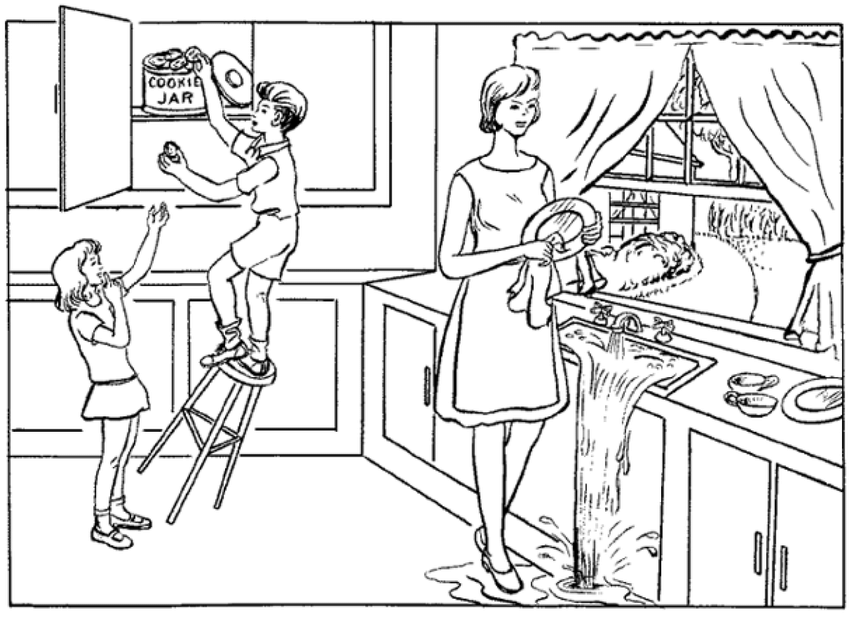
\includegraphics[width=0.4\textwidth]{figs/cookie_theft.png}
%   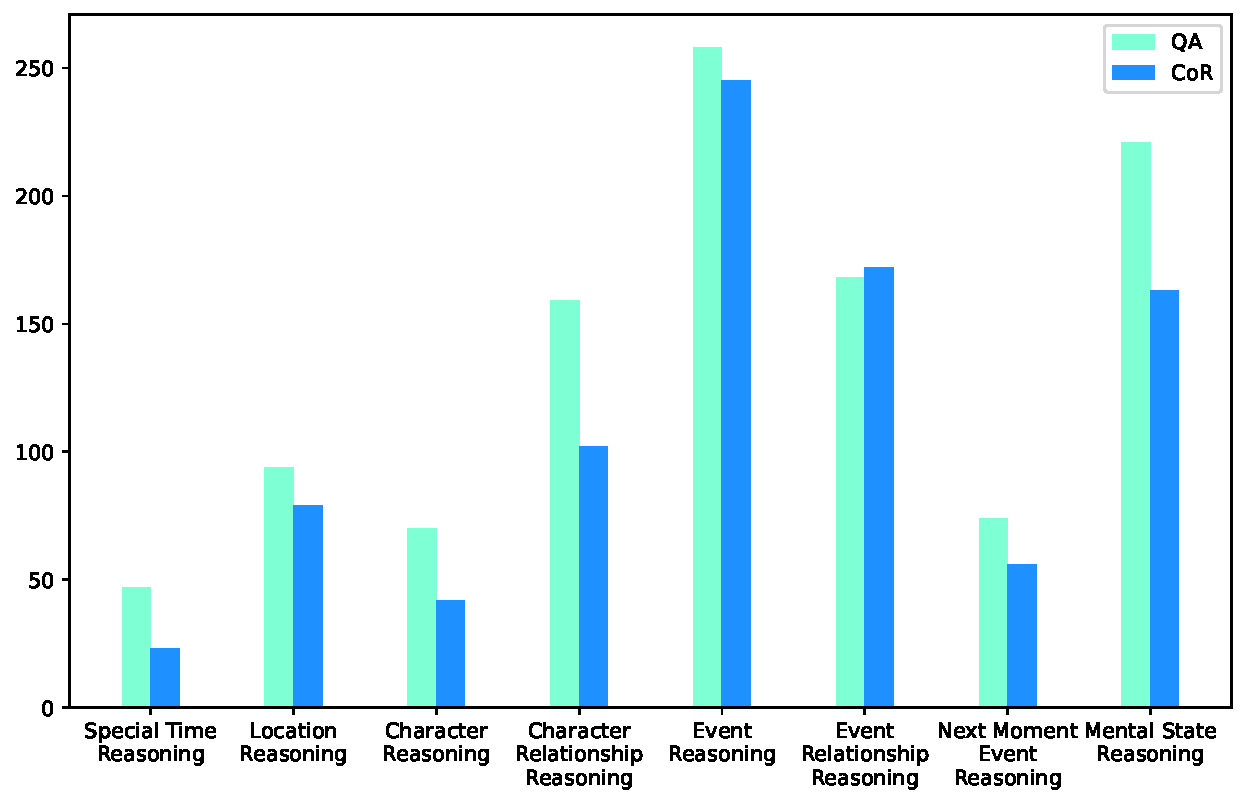
\includegraphics[width=0.48\textwidth]{figs/cogbench_stat.pdf}
%   \caption{Distribution of CoRs and questions in CogBench. \KZ{Fonts are
% too small. I repeat: text in figures and tables must be at least 2/3 of
% the size of main text.} \MY{Tables might be more suitable to show this stat. }}
%   % \footnote{https://dementia.talkbank.org/}
%   \label{fig:cogbench_stat}
% \end{figure}


\begin{table*}[th]
  \centering
  \small
  \setlength{\tabcolsep}{2.5pt} 
  \begin{tabular}{lcccccccc}
  \hline
  \textbf{} & \thead{\textbf{Time} } & \thead{\textbf{Location} } & \thead{\textbf{Character} } &  \thead{\textbf{Character}\\ \textbf{Relationship} } & \thead{\textbf{Event} } & \thead{\textbf{Event} \\ \textbf{Relationship} } & \thead{\textbf{Next Moment} \\ \textbf{Event} } & \thead{\textbf{Mental State} } \\ % \\ \textbf{Accuracy}
  \hline
  CoR & 23 & 79 & 42 & 102 &  245 & 172  & 56 & 162 \\
  QA & 47  & 94 & 70 & 159 & 258   &  168  & 74 & 221 \\  
  \hline
  \end{tabular}
  \caption{\label{tab:stat}
  Distribution of CoRs and questions in CogBench.
  }
\end{table*}

% Note that this is the first version of CogBench and we will keep updating CogBench and collect more high-quality images and annotations in the future.

% Each image requires one or more reasoning capabilities to understand.

% The reasons are as follows:

% Our data collection requirements are strict, so there are few high-quality images that meet the criteria. We aim to substitute quantity with high-quality images and annotations. Moreover, the cost of calling LLM API or using open-source MLLM inference is relatively high, so we expect to design a smaller, more user-friendly yet effective evaluation benchmark.


\subsection{Tasks in CogBench}

% As Cookie Theft is inherently utilized via picture description task, we adopted this task as the generative task in CogBench.
To comprehensively evaluate cognitive abilities of LVLMs, we designed a generative Image Description task and a discriminative Multiple-Choice Question Answering task in CogBench.

\subsubsection{Image Description Task}



% In Vision Language field, 
% Image captioning task is a classical task that requires models to generate a caption for an image. 
% The caption is usually a sentence that describes the image. 
% with the development of LLMs and LVLMs,
Inspired by Cookie Theft picture description task, we propose to assess the cognitive abilities of LVLMs through an Image Description task using Cookie Theft-like images.
Recently, some researchers \cite{xie2022visual, zhu2023chatgpt, zhuge2023mindstorms} are also trying to improve model performance on image description task. 
The difference between our description task and existing image description task is that we expect LVLMs understand and describe the story in the image through high-level cognitive reasoning. 
% The difference between CogID and existing image description task is that we mainly focus on evaluating high-level cognitive reasoning reflected in the description and the description tells a story.
% ability of LVLMs.
For instance, in Figure \ref{fig:cogbench}, the description of the image should not only include what is in the picture but also focus on elucidating the story of ``parents are going out to attend a formal event, and the mother is refusing the boy to accompany them'' through a series of reasonings.

% The fine-grained categories of reasoning we concern will be introduced in detail in Section \ref{sec:annotation}.
% \KZ{You should put an example of this task here, rather than in the figure.
% I think the figure should only contain the picture and maybe the
% description (no need to be complete).}
% \XJ{example added}



% expect LVLMs can recognize the entities in the image and reason about time, location, events, characters, mental states etc. in the image.

\subsubsection{Visual Question Answering Task}

% Since CogID is a generative task, 
% To comprehensively evaluate the cognitive ability of LVLMs and simplify evaluation, 
% The discriminative task we desgin in CogBench is named as Cognitive Visual Question Answering (CogVQA). 
% \KZ{The prev sentence is useless.} \XJ{removed}
All questions in VQA task are Multiple-Choice Questions with four options, which simplifies evaluation.
Similar to Description task, the questions in VQA task are also related to high-level cognitive reasoning. 
For example, in Figure \ref{fig:qa_example}, we can ask question about the event ``What is the woman doing?'' or question about the cause of the event ``Why is the mom placing her hands on the boy's forehead?'', which require models to answer with reasoning.
% \KZ{Give an example of the CVQA task here. Your description of
% these tasks are too dry!}
% \XJ{example added}
% This simplifies the evaluation process and makes it easier to evaluate the performance of models.
% With this task setting, the evaluation of CogVQA is more straightforward compared to CogID task and can help us evaluate the understanding of a LVLM of an image more directly and easily.
% We will introduce the question generation process in Section \ref{sec:question_generation}.

\begin{figure}
  \centering
  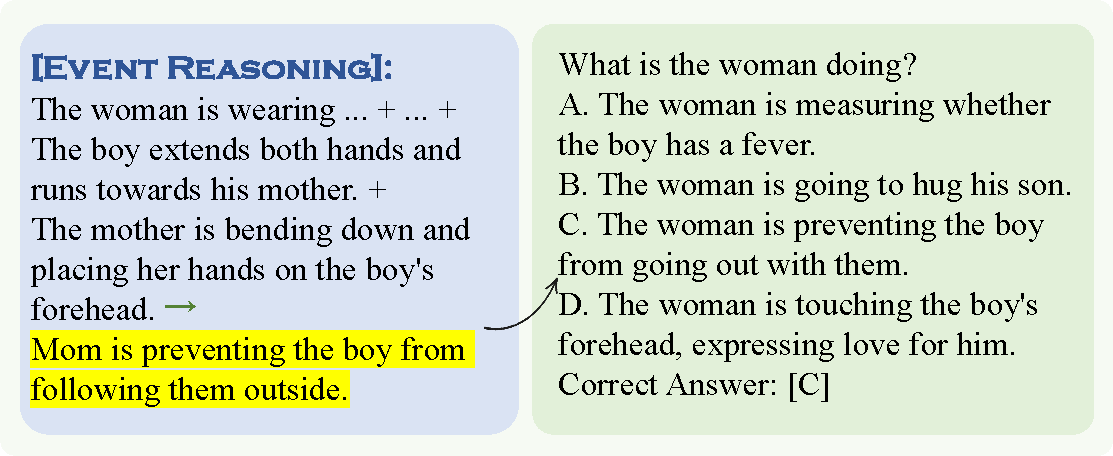
\includegraphics[width=0.5\textwidth]{figs/vqa_task_3.pdf}
  \caption{An example of VQA task from CogBench. 
}
  \label{fig:qa_example}
\end{figure}

% \subsubsection{CoR-based GPT-assisted Question Generation}
% \label{sec:question_generation}

% For the VQA task,
We use a semi-automatic GPT-assisted approach to generate questions for images based on [CoRs] we annotated in the previous section, referred to as CoR-based GPT-assisted Question Generation. 
% \KZ{This section
% includes too many acronyms.} 
The main idea of the question generation is that for each CoR, we can ask questions about both the conclusion (right part of $\rightarrow$) and reasons to draw the conclusion (left part of $\rightarrow$), as shown in Fiure \ref{fig:qa_example}. 
The process can be divided into two stages.

In the first stage, we use GPT-4 \cite{openai2023gpt4} to generate questions for images in CogBench. 
For each category of reasoning capability, we design a sepcific prompt for GPT-4 to generate questions, so that questions related to different types of CoRs can be generated.
For Question Generation, the key point is to generate high quality distractors. 
Thus, we encourage GPT-4 to hallucinate to generate more perplexing distractors in our prompt. 
Appendix \ref{sec:qa_prompt} shows an example of prompt we use for GPT-4 to generate questions.

Though GPT-4 is powerful, it is still difficult for it to generate 100\% satisfying questions for all images.
Thus, in the second stage, we manually select and modify the questions generated by GPT-4.
The principle of selection and modification is that the question cannot apparently point to the correct option and distractors should be as closely related to the question and the correct option as possible, thereby possessing a certain level of misleadingness.
During selection, ChatGPT is also utilized to help detect those simple questions that can be easily answered without having to accept the image as input. 
% \MY{do you have a number saying how many questions are rephrased? or all questions are human proof-read? On what standard? how to control the difficulty of the generated options in QA?}
% \XJ{Sorry, did not keep the number... standard added.}



